
\section{Galaxy Evolution}
\label{sec:galaxy_evolution}



%%%%%%%%%%%%%%%%%%%%%%%%%%%%%%%%%%%%%%%%%%%%%%%%%%%%
\subsection{Dark Matter Halos}

Every galaxy resides inside a dark matter halo.  Often about an order of magnitude larger in both radius and mass than the baryonic component, dark mater halos dominate the large-scale behavior of galaxies.  Dark matter is matter that is thought to interact very weakly or not at all with light and ordinary matter, except gravitationally.  Evidence for dark matter comes from a number of sources, including the relatively flat rotational velocity curve of galaxies, the velocity dispersion of galaxies, gravitational lensing measurements, galaxy clustering, and the offset between the gas and dominant mass measured in the Bullet cluster.  Here we will briefly discuss the evidence from flat rotation curves.

If there were no dark matter component and only the baryonic components (i.e. stars and gas) contributed to the galactic potential, we would expect the rotational velocity of galaxies to fall off with radius.  However, observations show that the rotation curve remains relatively flat \citep{rubin_1980}.  Figure \ref{fig:rotation_curves} shows several observed rotation curves.

\begin{figure}[H]
\centering
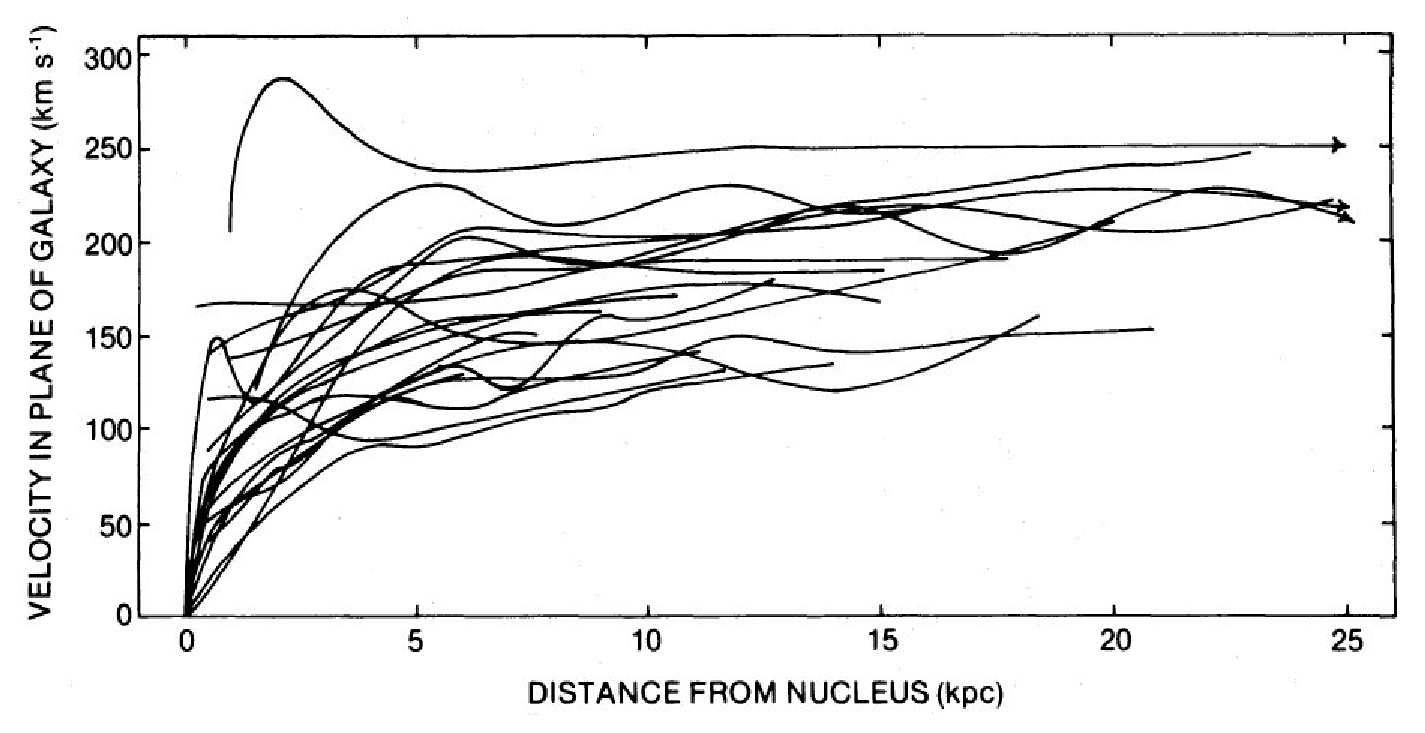
\includegraphics[width=\linewidth]{rubin_1980_rotation_curve.eps}
\caption[Rotation curves for 21 Sc galaxies]{\footnotesize Rotation curves for 21 Sc galaxies.  It is readily identifiable that the rotation curves do not fall off as would be expected for galaxies without a dark matter component.  \citep{rubin_1980}}
\label{fig:rotation_curves}
\end{figure}

\citet{navarro_1997} found that dark matter halos generally follow the same density profile, regardless of mass.  This universal dark matter density profile can be given as
\begin{equation} \label{nfw_profile}
  \rho(r) \propto \frac{1}{(r/a)(1+r/a)^{2}},
\end{equation}
where $a$ is the radius where the profile transitions from an $r^{-1}$ power law to an $r^{-3}$ power law.



%%%%%%%%%%%%%%%%%%%%%%%%%%%%%%%%%%%%%%%%%%%%%%%%%%%%
\subsection{Galaxy Mergers}

Galaxy mergers are the fundamental mechanism by which galaxies grow and evolve.  Collisions between galaxies trigger processes that can alter nearly all the properties of the galaxies.  Naturally, mergers increase the mass of galaxies.  Starting from small perturbations in the early universe, gravity slowly pulls matter together to form larger and larger clumps.  These clumps of gas and dark matter eventually form stars, beginning what we think of as typical galaxies, and over time, these galaxies merge together into larger and larger galaxies.

Mergers affect many other properties of galaxies as well.  Mergers distort the shapes of galaxies, causing long tidal tails to form and the entire morphology to appear irregular.  The disk structures of spiral galaxies that form from the settling of the rotational component are distorted and ``puffed up'' into components with ever increasing bulge-like properties.

Mergers can trigger wide-scale starburst events, where a large portion of gas goes into the formation of stars.  Much of the gas component of the galaxy can subsequently be blown out by the winds from the supernovae of short-lived O and B stars.  This shuts off star formation, and as the stellar population is no longer replenished with new high-mass stars, the galaxy becomes progressively redder as large stars die.

The general trend is for mergers to move galaxies from the right side of the Hubble tuning fork towards the left, turning blue, gas rich spirals into red, gas poor ellipticals.  This process is aided by the AGN feedback also triggered during galaxy mergers, as we discuss in the following section.



%%%%%%%%%%%%%%%%%%%%%%%%%%%%%%%%%%%%%%%%%%%%%%%%%%%%
%\subsection{Gas Content and Stellar Populations}

%!!! Add content about the evolution of gas content and stellar populations.



